\documentclass{article}
\usepackage[margin=3cm]{geometry}
\usepackage[utf8]{inputenc}
\usepackage{amsmath}
\usepackage{amssymb}
\usepackage{float}
\usepackage{enumitem}
\usepackage{graphicx}
\usepackage{caption}
\usepackage{subcaption}

\title{Nonlinear Optimization - Homework 1 }
\author{Christian Segercrantz 481056}

\begin{document}
	\maketitle
	\pagebreak
\section*{1.1}
	%First non-empty and convex
	%Theorem 2
	% ξ > (x − x) ≥ 0 for all x ∈ S
	We will first examine weather the set is non-empty and convex. 

\section*{1.2}
\section*{1.3}
\section*{1.4}

\begin{figure}[H]
	\centering
	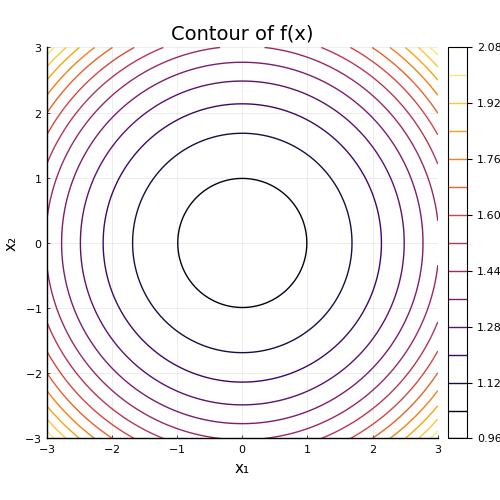
\includegraphics{plots/1_4c_contour.png}
	\caption{Capion here}
	\label{fig:1.4c}
\end{figure}

\end{document}